\chapter{Design}
\label{chapter:Design}
%Overarching design in a top-down view: 
%-server/client design overall architecture, system model
%-describe file system, 
%-how protocol is peformed by the server
%-describe current functionality of the implementation. Handles protocol run, view-changes and checkpointing

%old version:-overall usage over different parameters, overaching stuff thats not the actual implementation of the algorithm, but the network layer to server to algorithm, how to run the algorithm/checkpointing/view changes.
%first draft!!!
This chapter present an overall summary of the PBFT application implemented. This includes a brief summary of the system model used for performing the PBFT algorithm. The structure of the application including a brief introduction to its file structure as well as describing the general design for performing the consensus algorithm. We will finally describe the current functionalities that are present in the current application. 

\section{System Model}
\begin{figure}
	\centering
	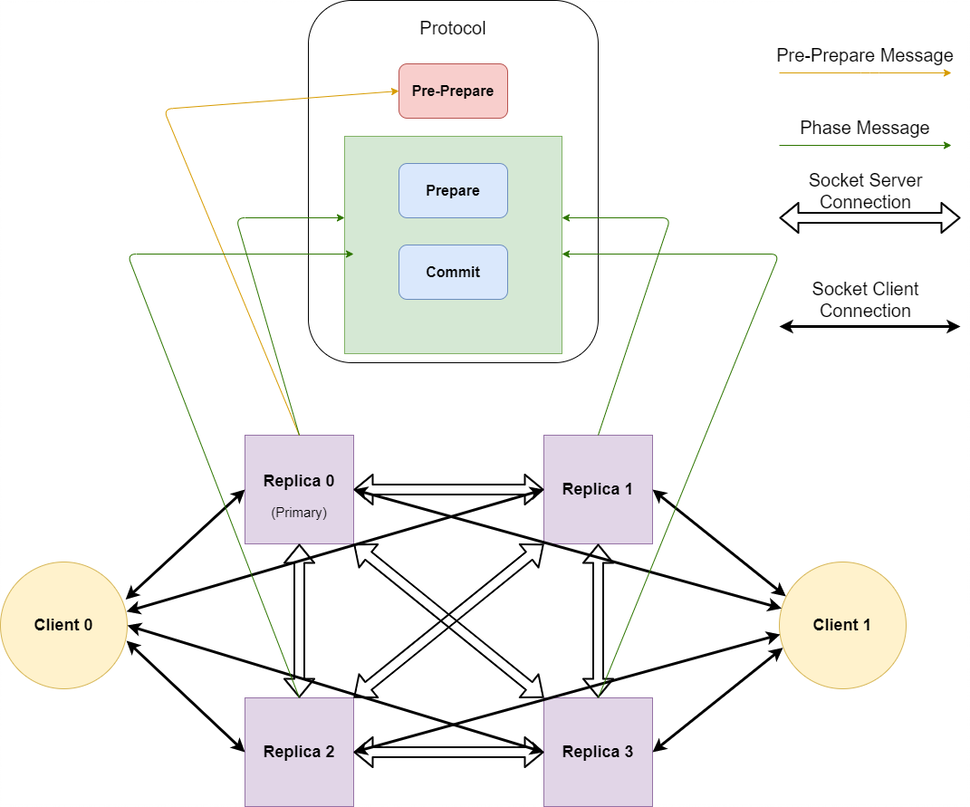
\includegraphics[width=\linewidth]{figures/meshnetwork}
	\caption{Overall architecture of the PBFT implementation networking}
	\label{fig:meshnetwork}
\end{figure}
The figure \autoref{fig:meshnetwork} shows the system model used for PBFT implementation. Generally our system model follows the same structure as the system model introduced in the PBFT chapter\autoref{sec:systemModel}. The system consist of four server implementations called \emph{replicas}, where the replica with the lowest identifier value is chosen as the primary. These four replicas are communicating over a mesh network using socket connections. This means each replica shares an unique network socket with each other replica in the PBFT network. In order to avoid creating multiple socket connections between replicas, the replica with the highest identifier is the one tasked with being the initiator when it comes to establishing a socket connection between other replicas. Meaning for instance that the primary replica, will not need to actively establish any connections to its fellow replicas. The primary will instead establish all of its socket connections by listening for any connections attempts on its local network address. The opposite scenario occurs for the replica with the highest identifier value, although the replica still listens for connections on its local network address, it is also responsible for establishing the connections with all the other replicas in the network with lower identifier values.

Even when the replicas have established connections, the replicas can not fully communicate with each other until they have exchanged public keys. This is required in order to verify messages sent by each replica using a digital signature. Public keys are exchanged in \emph{session messages}, which are messages that are automatically sent between parties once a socket connection has been established. If the public keys are for some reason not exchanged, than the replica will discard any message received from that host and thereafter terminate the connection. This also applies for clients. This current model is unfortunately not very secure, due to public keys being ephemeral and are intended to be replaced in the case of a crash occurring. Currently in this implementation, the private and public key pair for a replica are randomly created at the system start-up. Considering there is currently no way for the replicas to authenticate another replica after reboot, it will replace the key value pair currently in the register if a new session message with the same identifier value is received. This in turn means the system is susceptible to impersonation and spoofing attacks. Since the main goal of this thesis was more focused on the implementation of the PBFT workflow, this cryptographic system was deemed sufficient for simulating a network using digital signatures. However, it is important to be aware of this flaw in the system in order to avoid this issue in the future. %add how to fix this in future work.

The system performs the PBFT protocol by exchanging protocol messages over the mesh network until atleast three of the servers have finished all three protocol phases. In this implementation protocol messages are referred to as \emph{phase messages}. The PBFT protocol is trigger when the server receives a request from one of the connected client nodes. The primary is responsible for officially starting an instance of the PBFT protocol by multicasting a phase message of type pre-prepare. There are two important goals for the pre-prepare phase. The first is to make sure that the replicas have an agreement upon the ordering of the request. In other words, the replicas will perform the requests in the same order as the primary, which in turn means the request should have the same sequence numbers throughout the network. The second important goal is to determine whether or not the primary is fit to be leader. As mention in section \autoref{sec:view-change}, a view-change occurs when a leader no longer is eligible. In our application the view-changes are triggered by timeout which are set once a replica receives a client's request. If the primary takes too long in the pre-prepare phase, than the timeout will exceed and the other replicas will perform a view-change in order to change the primary replica. Although it would be useful to have timeouts in the commit phase in the instance where majority of servers are unable to properly finish the commit phase, it is currently not supported in our implementation due to how timeouts are handled inside the protocol workflow(should probably be moved elsewhere). The rest of the replicas will be the responsible party during the prepare phase by sending phase messages of type prepare, while every replica will participate in the commit phase using commit type phase messages. The last step of current PBFT implementation is to create a reply message and send it back to client responsible for the request. The details in regards to how the PBFT workflow is currently being handled will be discussed in the next chapter \autoref{chapter:Imp}.

\section{File structure}
In figure we \autoref{fig:filestruct} can see a short summary of the file system used in a PBFT replica system. The summary shows each of the root folders as well as the most important files. To start of the folders \emph{Messages} and \emph{Certificates} contains all the message types and certificate types available for this implementation. This includes files containing the interfaces. The \emph{Helper} folder contains all the static functions used in the PBFT implementation that are not linked to any specific object instance. This includes functionality for serializing and deserializing messages objects with JSON, cryptographic functions related to creating and validating digital signatures and files containing all the enum types used for this thesis. An enum is ... ~\cite{WEB:Enum}.

\newpage
\begin{wrapfigure}{r}{0.45\linewidth}
\centering
%\vspace{15pt}
%\rule{0.9\linewidth}{0.75\linewidth}
% ,scale=0.8, every node/.style={scale=0.8}
\tikzstyle{every node}=[draw=black,thick,anchor=west]
    \begin{tikzpicture}[%
      grow via three points={one child at (0.5,-0.7) and
      two children at (0.5,-0.7) and (0.5,-1.4)},
      edge from parent path={(\tikzparentnode.south) |- (\tikzchildnode.west)}]
      \node {PBFT}
        child { node {App.cs}}
        child { node {Certificates}
        	child {node {...}}
        	}	
        child [missing] {}
        child { node {Messages}
        	child {node {...}}
        	}
        child [missing] {}
        child { node {Helper}
        	child {node {...}}
        	}
        child [missing] {}
        child { node {JSONFiles}
        	child {node {serverInfo.json}}
        	child {node {testServerInfo.json}}
        	}
        child [missing] {}
        child [missing] {}
        child { node {Storage}
        	child {node {...}}
        }
        child [missing] {}
        child { node {Replica}
          child { node {Server.cs}}
          child { node {Network}
          	child {node {...}}
        	}
        }
        child [missing] {
          child { node {Protocol}
          child { node {Workflow.cs}}
          child { node {...}}
        	}
        };
\end{tikzpicture}
    \caption{Summary of the file architecture for the PBFT implementation}
    \label{fig:filestruct}
    \vspace{40pt}
\end{wrapfigure}

\section{Server and protocol interaction}

\begin{figure}
	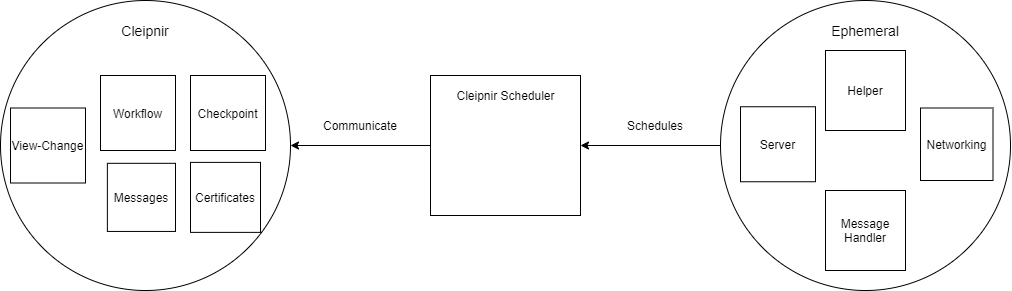
\includegraphics[width=\linewidth]{figures/CleipnirStructurever1}
	\caption{Application divided into persistent parts and ephermeral parts and how they interact}
	\label{fig:PersistencyEphemeral}
\end{figure}